%% introduction to the book
\chapter{Introduction to the topic of this book}
\label{ch:intro}

\begin{quote}
  \itshape \foreignlanguage{ngerman}{Poincar\'e sagte gelegentlich,
  dass alle Mathematik eine Gruppengeschichte war.
  Ich erz\"ahlte ihm dann \"uber dein Programm,
  das er nicht kannte.}

  \smallskip

  \noindent Poincar\'e was saying
  that all of mathematics was a tale about groups.
  I then told him about your program,
  which he didn't know about.
\end{quote}
\hfill (Letter from Sophus Lie to Felix Klein, October 1882)

\bigskip

%{\em If this book is about group theory, then here we will explain what's interesting about groups and why one would want to study them.}


Since this book is called ``Symmetry'' it is reasonable to hope
that by the time you've reached the end you'll have a clear idea of
what symmetry means.

Ideally the answer should give a solid foundation for dealing with
questions about symmetries. It should also equip you with language
with which to talk about symmetries, making precise -- but also
reflecting faithfully -- the intuition humans seem to be born with.

So, we should start by talking about how one intuitively can approach the
subject while giving hints about how this intuition can be made into
the solid, workable tool, which is the topic of this book.

\sususe{What is symmetry?}

When we say that something is ``symmetric'' or possesses many ``symmetries'',
we mean that the thing remains unchanged, even if we ``do things to it.''
The best examples to begin with is if the something is some shape, for
instance this square $\square$. Rotating by 90 degrees doesn’t change it, so we may say that ``rotation by 90 degrees is a symmetry of $\square$''
Of course, rotating by $90$ degrees will move individual points in $\square$, but that
is not of essence -- the shape remains the same.
However, the outcome of rotating by $360$ degree or not at all
is the same - even from the point of view of each individual point in $\square$ -- so it probably feels contrived to count rotations by $0$ and $360$ degrees as different rotations.

It feels reasonable to consider the rotations by $0$\textdegree, $90$\textdegree, $180$\textdegree, and $270$\textdegree{} to be all the (rotational) symmetries of $\square$.  Two thoughts may strike you:
\begin{enumerate}
\item
  are these \emph{all} the symmetries?
\item ``rotation'' indicates a \emph{motion}, through different squares,
joining $\square$ with itself via a ``journey in the world of squares''.

The following cartoon animates a rotation of $\square$ by $90$\textdegree.
The center of the square should be thought of as being in the same place
all the time.
\end{enumerate}
\begin{center}
  \begin{tikzpicture}
    \foreach \x/\s in {45/0,35/1,25/2,15/3,5/4,-5/5,-15/6,-25/7,-35/8,-45/9} {
      \begin{scope}[xshift=\s cm]
        \draw (\x:.3) -- (\x+90:.3) -- (\x+180:.3) -- (\x+270:.3) -- cycle;
      \end{scope}
    }
    % stick figure pushing
    \begin{scope}[thick,line cap=round]
      \node[dot] at (-.3,.3) {};
      \draw (-.4,.1) -- (-.212,.1);
      \draw (-.5,-.1) -- (-.35,.2);
      \draw (-.5,-.1) -- (-.35,-.1);
      \draw (-.5,-.1) -- (-.6,-.2);
      \draw (-.35,-.1) -- (-.38,-.3);
      \draw (-.38,-.3) -- (-.33,-.3);
      \draw (-.6,-.2) -- (-.78,-.28);
      \draw (-.78,-.28) -- (-.73,-.3);
    \end{scope}
    % stick figure resting
    \begin{scope}[thick,line cap=round,xshift=9cm]
      \node[dot] at (.5,.35) {};
      \draw (.5,.25) -- (.5,-.05);
      \draw (.5,-.05) -- (.6,-.3);
      \draw (.6,-.3) -- (.65,-.3);
      \draw (.5,-.05) -- (.4,-.3);
      \draw (.4,-.3) -- (.35,-.3);
      \draw (.5,.25) -- (.65,.1);
      \draw (.65,.1) -- (.5,-.02);
      \draw (.5,.25) -- (.35,.15);
      \draw (.35,.15) -- (.212,.212);
    \end{scope}
  \end{tikzpicture}
\end{center}
How is that reconcilable with a precise notion of symmetry?

The answer to the first question clearly depends on the context. 
For example, if we allow reflections the answer is ``no''.
Each context has its own answer to what the symmetries of the square are.

Actually, the two questions should be seen as connected. 
If a symmetry of $\square$ is like a round trip (loop) 
in the world (type) of squares, what symmetries are allowed is 
dependent on how big a ``world of squares'' we consider. 
Is it, for instance, big enough to contain a loop representing a reflection?

We argue that in order to pin down the symmetries of a thing (a ``shape''), all you need to do is specify
\begin{enumerate}
\item a type $X$ (of things), and
\item the particular thing $x$ (in $X$).
\end{enumerate}
It is (almost) that simple!

Note that this presupposes that our setup is strong enough to support the
notion of a round trip.

\sususe{From ``things'' to mathematical objects}

Different setups have different advantages.
The theory of sets is an absolutely wonderful setup, but supporting the
notion of a round trip in sets requires at the very least developing fields
like \emph{mathematical analysis}, \emph{topology} and \emph{homotopy theory},
which (while fun and worthwhile in itself) is something of a detour.

The setup we adopt, homotopy type theory, or univalent foundations, 
seems custom-built for supporting the notion of a round trip of
a thing $x$ in a type $X$. 
We get support for important operations on round trips
of $x$: one can do such round trips after another (composition),
one can go any round trip in the reversed direction (inverse), and there
is always the trivial round trip of staying in place (unit).
This provides round trips with a structure that is called a \emph{group}
in mathematics, satisfying all the properties that these operations
ought to have. 

In practice, one of the most important things is to be able to \emph{compare}
symmetries of ``thing~1'' and ``thing~2''. 
In our case this amounts to nothing but a function, $f: X_1 \to X_2$, 
that takes thing~1, $x_1$ in $X_1$, to thing~2, $x_2$ in $X_2$.
\begin{center}
\begin{tikzpicture}
  \begin{scope}[scale=0.8]
    \node (X) at (1,2) {$X_1$};
    \draw (0,-2)
    .. controls ++(150:-1) and ++(180:1) .. (3,-2)
    .. controls ++(180:-1) and ++(-100:1.3) .. (4.5,0)
    .. controls ++(-100:-1.3) and ++(-10:2) .. (2,1.5)
    .. controls ++(-10:-2) and ++(90:1) .. (-1,0)
    .. controls ++(90:-1) and ++(150:1) .. (0,-2);
    \node[dot,casred,label=left:$x_1$] (x1) at (0,0) {};
    \draw[->,casblue] (x1) .. controls ++(80:-1) and ++(170:1) .. (.5,-1.5)
    .. controls ++(170:-1) and ++(200:1) .. (3,-1.4)
    .. controls ++(200:-1) and ++(-80:.5) .. (3.8,0)
    .. controls ++(-80:-.5) and ++(-10:.3) .. (3,1)
    .. controls ++(-10:-.3) and ++(80:1) .. (x1);
    \draw (1,-1) arc(210:330:.8 and .5);
    \draw (2.09,-1.18) arc(60:120:.8 and .7);
    \draw (1.5,0) arc(210:330:.8 and .5);
    \draw (2.59,-0.18) arc(60:120:.8 and .7);
    \draw[->] (4.8,0) -- node[auto] {$f$} (6.3,0);
  \end{scope}
  \begin{scope}[xshift=6cm,scale=0.8]
    \node (X) at (1,2) {$X_2$};
    \draw (0,-1)
    .. controls ++(200:-1) and ++(180:1) .. (2,-2)
    .. controls ++(180:-1) and ++(270:1) .. (4,0)
    .. controls ++(270:-1) and ++(20:2)   .. (2,2)
    .. controls ++(20:-2)   and ++(90:1)  .. (-1,0)
    .. controls ++(90:-1)  and ++(200:1) .. (0,-1);
    \node[dot,casred,label=below:$x_2$] (x2) at (0,0) {};
    \draw[->,casblue] (x2) .. controls ++(-20:1.5) and ++(170:1) ..
      (2,-1) .. controls ++(170:-1) and ++(-70:1) ..
      (3.1,0) .. controls ++(-70:-1) and ++(90:.5) ..
      (3.5,0) .. controls ++(90:-.5) and ++(-120:2) ..
      (3,1) .. controls ++(-120:-2) and ++(-20:-1.5) .. (x2);
    \draw (1,0) arc(210:330:.8 and .5);
    \draw (2.09,-.18) arc(60:120:.8 and .7);
  \end{scope}
\end{tikzpicture}
\end{center}
While such comparisons of symmetries are traditionally handled by something called a \emph{group homomorphism} which is a function satisfying a rather long list of axioms, in our setup the only thing we need to know of the function is that it really does take thing~1 to thing~2 -- everything else then follows naturally.

Some important examples have provocatively simple representations in
this framework.  For instance, consider the circle shown in the margin,
with one designated point $x$ on it.\marginnote{%
  \begin{tikzpicture}
    \node[dot,label=right:$x$] (base) at (1,0) {};
    \draw (0,0) circle (1);
  \end{tikzpicture}}
Since symmetries of $x$ are interpreted as loops, you see that you have a loop for every integer -- the number $7$ can be represented by looping seven times counterclockwise.  As we shall see, in our setup any loop in the circle is naturally identified with a unique integer (the \emph{winding number} if you will).  Everything you can wish to know about the structure of the \emph{group of integers} is built-in in the circle.

Another example is the \emph{free group of words in two letters $a$ and $b$}.  This is represented by the figure eight in the margin.\marginnote{%
  \begin{tikzpicture}
    \node[dot,label=right:$x$] (base) at (1,0) {};
    \draw (0,0) circle (1);
    \draw (2,0) circle (1);
    \node (a) at (-.9,.9) {$a$};
    \node (b) at (2.9,.9) {$b$};
  \end{tikzpicture}}
In order to be able to distinguish the two circles we call them $a$ and $b$,
with the point $x$ as the (only) point on both.
The word $ab^2a^{-1}$ is represented by looping around circles $a$ and $b$ respectively $1$, $2$ and $-1$ times in succession -- notice that since the $b^2$ is in the middle it prevents the $a$ and the $a^{-1}$ from meeting and cancelling each other out.  If you wanted the \emph{abelian} group on the letters $a$ and $b$ (where $a$ and $b$ are allowed to move past each other), you should instead look at the torus:
\begin{center}
\begin{tikzpicture}
  \useasboundingbox (-3,-1.5) rectangle (3,1.5);
  \begin{scope}[xshift=2.4cm,yshift=.35cm,xscale=cos(25)]
  \draw[casred,line cap=round] (0,0) arc (65:148:0.7);
  \draw[casred] (0,0) arc (65:-40:0.7);
  \end{scope}
  \draw[casblue] (0,.35) ellipse (2.4 and 0.9);
  \draw (0,0) ellipse (3 and 1.5);
  \begin{scope}
    \clip (0,-1.8) ellipse (3 and 2.5);
    \draw (0,2.2) ellipse (3 and 2.5);
  \end{scope}
  \begin{scope}
    \clip (0,2.2) ellipse (3 and 2.5);
    \draw (0,-2.2) ellipse (3 and 2.5);
  \end{scope}
  \node[dot] at (2.4,0.35) {};
  \node (a) at (2.6,-.2) {$a$};
  \node (b) at (0,1) {$b$};
\end{tikzpicture}
\end{center}
Just why this last example works can remain a puzzle for now.

\sususe{The importance of the ambient type $X$ ``of things''}

In many situations, the type $X$ ``of things'' can be more difficult to draw,
or to define mathematically.  For instance, what is the ``type of all squares'' which we discussed earlier, representing all rotational symmetries of $\square$?  You have perhaps already visualized it as the type of all squares in the plane, with $\square$ being the shape the loop must start and stop in. This idea works well for the \emph{oriented square} depicted\marginnote{%
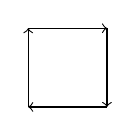
\begin{tikzpicture}
\draw[->] (0,0) -- (0,1);
\draw[->] (0,1) -- (1,1);
\draw[->] (1,1) -- (1,0);
\draw[->] (1,0) -- (0,0);
\end{tikzpicture}
}
in the margin. Note that the only reflective symmetry of the oriented
square is reflection in the center -- and the outcome is the same
as a rotation by $180$\textdegree. However, for $\square$ we would get
reflective symmetries that are not rotations.
It is actually a little difficult to come
up with a simple geometry of the plane that gives exactly the rotational
symmetries of $\square$. Later in the book, we will first pursue an
algebraic approach, using that any rotational symmetry of $\square$
can be reached by doing the $90$\textdegree-rotation a few times, 
together with the fact that taking any loop four times reduces to not doing
anything at all: they represent the \emph{cyclic group of order four}.

A by-product of this line of thinking is the distinguished position of the circle. To express this it is convenient to give names to things: let $\base$ (\ie a dot) be the chosen base point in the circle and $\Sloop$ the loop winding once around the circle counterclockwise. Then a symmetry of a shape $x_0$ in $X$ is uniquely given by the image of $\Sloop $ under a function $\Sc\to X$ taking $\base$ to $x_0$. So,
\begin{quote}
  the study of symmetries is the study of (pointed) functions between types of things, with the circle being the type that gives you access to individual symmetries.
\end{quote}

This is similar to the idea of replacing membership in a set $S$ by function from a one-point set $1$ into $S$: a point $s$ in $S$ is uniquely given by the function $1\to S$ taking the value $s$.


Just as you don't need much information about the one-point set to get this to work, you don't need much information about the circle to embark on a study of symmetries.
Essentially you need to know of $\base $ and $\Sloop $, and that there is no ``hidden relation'' between the symmetries of $\base$. Contrast this to the type of squares which has such a ``hidden relation'': where we identified a $360$\textdegree\ rotation with doing nothing.  This point of view has the benefit of being readily formalized while offering geometric intuition.

\sususe{Symmetries have natural scopes}

The natural scope of the symmetries of a thing $x$ in a type $X$
are the things in $X$ that can be reached from $x$ by a journey in $X$.

Let's make this precise with an example.
In our setup,
as a consequence of univalence, journeys from one set to another
in the type of sets are
uniquely given by one-to-one correspondences between these sets,
commonly called \emph{bijections}.

Now consider the set $\{1,2,3\}$. Then a symmetry of $\{1,2,3\}$ in the type of finite sets amounts to the same thing as a symmetry of $\{1,2,3\}$ in the type of sets with three elements: a symmetry of $\{1,2,3\}$ will not ``pass through'' sets that have, say, five elements. Think of the type of finite sets as being the disjoint union of all the types of sets with $n$-elements, where $n=0,1,2,\dots$: if a symmetry is a loop it should not be allowed to jump between the type of sets with three elements and the type of sets with five elements.\marginnote{%
  Type of empty sets:\\
  \begin{tikzpicture}
    \draw plot [smooth cycle] coordinates {(0,0) (3,-.5) (3.5,1) (1,2)};
    \node[dot,label=above right:{flying elephants}] (fe) at (.5,0) {};
    \node[dot,label=below:{live dodos}] (ld) at (2,1.5) {};
    \node at (1,0.75) {$\cdots$};
  \end{tikzpicture}\\
  Type of one-element sets:\\
  \begin{tikzpicture}
    \draw plot [smooth cycle] coordinates {(0,-.5) (3,0) (3.5,2) (1,1)};
    \node[dot,label=above:{$\{1\}$}] (one) at (1,0) {};
    \node[dot,label=below:{$\{\text{Calvin}\}$}] (calvin) at (2.5,1.3) {};
    \node at (2,0.25) {$\cdots$};
  \end{tikzpicture}\\
  Type of two-element sets:\\
  \begin{tikzpicture}
    \draw plot [smooth cycle] coordinates {(0,1) (1,-1) (3.7,-.5) (3.5,2) (1.5,1.5)};
    \node[dot,label=above:{$\{1,2\}$}] (onetwo) at (.5,.5) {};
    \node[dot,label=below:{$\{\text{Calvin},\text{Hobbes}\}$}]
      (calvinhobbes) at (2.5,1.5) {};
    \node[dot,label=below:{$\{9,\text{Louise}\}$}] (ninelouise) at (3,0.5) {};
    \node[dot,label=above:{$\{\text{Thelma},\text{Hobbes}\}$}]
      (thelmahobbes) at (2,-0.8) {};
    \node at (1.5,0.2) {$\cdots$};
    \node at (1.5,-1.5) {$\vdots$};
  \end{tikzpicture}}

In fact, \emph{any} type $X$ can be naturally divided into ``components'': each
element $x_0$ in $X$ belongs to one and only one component, and the one $x_0$
belongs to we call $\conncomp X {x_0}$, and the symmetries of $x_0$ in $X$ may
be identified with the symmetries of $x_0$ in $\conncomp X {x_0}$. Hence from
the perspective of symmetries of $x_0$ only the component containing it matters,
and we confine our discussion to ``connected'' types of things, \ie those having
just one component.

The geometric intuition also points to the possibility of seemingly different symmetries being identified: when looping once around the circle it shouldn't matter ``how'' or ``how fast'' you do it. Consider the picture of the abelian group on two letters ${\color{casred}a}$ and ${\color{casblue}b}$ from before, but now together with a more frivolous loop (in pink) homotopic to $a$:
\begin{center}
\begin{tikzpicture}
  \useasboundingbox (-3,-1.5) rectangle (3,1.5);
  \begin{scope}[xshift=2.4cm,yshift=.35cm,xscale=cos(25)]
  \draw[casred!25] (0,0) arc (65:425:0.685);
  \draw[casred,line cap=round] (0,0) arc (65:148:0.685);
  \draw[casred] (0,0) arc (65:-55:0.685);
  \end{scope}
  \draw[orange] (2.4,0.35) .. controls ++(.1,-.5) and ++(.6,.3) .. (2,-1.12);
  \draw[orange!25] (2,-1.12) .. controls ++(-.6,-.3) and ++(-.5,-.2) .. (1.21,-0.09);
  \draw[orange] (1.21,-0.09) .. controls ++(.5,.2) and ++(-.2,-.2) .. (2.4,0.35);
  \draw[casblue] (0,.35) ellipse (2.4 and 0.9);
  \draw (0,0) ellipse (3 and 1.5);
  \begin{scope}
    \clip (0,-1.8) ellipse (3 and 2.5);
    \draw (0,2.2) ellipse (3 and 2.5);
  \end{scope}
  \begin{scope}
    \clip (0,2.2) ellipse (3 and 2.5);
    \draw (0,-2.2) ellipse (3 and 2.5);
  \end{scope}
  \node[dot] at (2.4,0.35) {};
  \node (a) at (2.6,-.2) {$a$};
  \node (b) at (0,1) {$b$};
\end{tikzpicture}
\end{center}
You might think of a symmetries of $x_0$ as a rubber band confined to the circle
and pinned to $x_0$. In the picture we've drawn such a rubber band (in orange)
which can be deformed to $a$, and this deformation we consider as
an \emph{identification of the two symmetries}.  In the language we adopt, this
is hard-wired, and so our arguments are independent of any picture: pictures
serve only as inspirations and are very helpful when trying to discover
proofs.\footnote{There's a subtle point, which may be a source of
  confusion if brushed under the carpet: a priori there could be ``several
  ways'' in which two symmetries should be identified. For many purposes this
  poses no problem, but we want to present a theory that mirrors the classical
  theory faithfully, and so restrict our ``types of things'' where there aren't
  multiple ways of identifying symmetries. The technical term -- when we get
  that far will be ``pointed connected groupoids''. This means disallowing types
  like the sphere:
  \begin{center}
    \begin{tikzpicture}
      \draw (0,0) circle (1);
      \draw[casred] (0,0) ellipse (1 and .3);
      \node[dot,label=right:$x_0$] at (1,0) {};
    \end{tikzpicture}
  \end{center}
  There are fundamentally different ways of identifying the symmetry represented
  of $x_0$ by the equator with the trivial symmetry: when thought of as a rubber
  band the equator can contract either over the north or the south poles (or
  more complicated ways). There's something called ``truncation'' which can fix
  any type to one of the desired sort where identifications of symmetries are
  unique.}%endfootnote

Our use of univalent foundations has several advantages. Roughly, univalence is the assertion that two types are ``equivalent'' if and only if there is a ``path'' (called an ``identification'') between them in the (large) ``type of types''. In group theory, two groups share exactly the same properties if there is an ``isomorphism'' between them (an invertible homomorphism), and with univalent foundation this is manifested by the isomorphism corresponding to a path between the groups in the type of groups. Hence we can use this path to transport any theorem about one group to the other: the two groups are ``identified''. The power of univalence is hard to overstate; it will simplify many proofs and make many statements accessible that otherwise would have been out of reach.

There are many kinds of symmetry and many ways of studying it.
Euclidean plane geometry is the study of properties that are invariant under rigid motions of the plane.
Other kinds of geometry arise by considering other notions of transformation.
Univalent mathematics gives a new perspective on symmetries:
Motions of the plane are forms of identifying the plane with itself in possibly non-trivial ways.
It may also be useful to consider different presentations of planes
(for instance as embedded in a common three-dimensional space)
and different identifications between them.
For instance, when drawing images in perspective
we identify planes in the scene with the image plane,
not in a rigid Euclidean way, but
rather via a perspectivity (see~\cref{fig:perspectivity}).
This gives rise to projective geometry.
\begin{marginfigure}
  \begin{center}
    \footnotesize
    \begin{tikzpicture}
      \node[dot,label=left:$O$] (O) at (0,0) {};
      \node[dot,casred,label=below:$A$] (A) at (1,-.3) {};
      \node[dot,casblue,label=below:$A'$] (Ap) at (2,-.6) {};
      \node[dot,casred,label={[label distance=-1pt]-95:$B$}] (B) at (.8,.2) {};
      \node[dot,casblue,label=right:$B'$] (Bp) at (2.4,.6) {};
      \node[dot,casred,label=above:$C$] (C) at (1.05,.7) {};
      \node[dot,casblue,label=above:$C'$] (Cp) at (2.1,1.4) {};
      \draw[casred,fill=casred!25] (A.center) -- (B.center) -- (C.center) -- cycle;
      \draw[casblue,fill=casblue!25] (Ap.center) -- (Bp.center) -- (Cp.center) -- cycle;
      \draw[dashed] (O) -- (Ap.center);
      \draw[dashed] (O) -- (Bp.center);
      \draw[dashed] (O) -- (Cp.center);
    \end{tikzpicture}
  \end{center}
  \caption{A perspectivity identifies the planes determined by the triangles $ABC$ and $A'B'C'$ in a way that doesn't preserve Euclidean distances or angles.}
  \label{fig:perspectivity}
\end{marginfigure}

Does that mean that a plane from the point of view of Euclidean
geometry is not the same as a plane from the point of view of
projective or affine geometry?
Yes.
These are of different types,
because they have different notions of identification,
and thus they have different properties.

Here we follow Quine's dictum: No entity without identity!
To know a type of objects is to know what it means to identify representatives of the type.
The collection of self-identifications (self-transformations) of a given object form a \emph{group}.

% TODO : Propositions, sets, and $1$-types (groupoids). (Here?)

Group theory emerged from many different directions in the latter half of the 19\th century.
Lagrange initiated the study of the invariants under permutations
of the roots of a polynomial equation $f(x)=0$,
which culminated in the celebrated work of Abel and Galois,
proving the unsolvability of general quintic (and higher degree)
polynomials by radicals.
In number theory, Gauss had made detailed studies of modular arithmetic,
proving for instance that the group of units of
$\ZZ/n\ZZ$ is cyclic precisely when $n$ is $1$, $2$, $4$, $p^k$ or $2p^k$, where $p$ is an odd prime and $k > 0$.
Klein was bringing order to geometry by considering groups of transformation,
while Lie was applying group theory in analysis to the study of differential equations.

Galois was the first to use the word ``group'' in a technical sense,
speaking of collections of permutations closed under composition.
He realized that the existence of a resolvent equation is equivalent
to the existence of a normal subgroup of prime index
in the group of the equation.

\subsection{Who is this book for?}
\label{sec:who}
At the outset the plan for this book was that it ought to cater for two very groups of readers. If you already have a classical first course in abstract group theory, this text has as its ambition that you should gain a new perspective on the material, \emph{and at the same time} learn about homotopy type theory by seeing it applied to a field you are familiar with. However, at the outset, another audience seemed just as plausible to us: what if you're not well versed in abstract algebra, but open to learning about it from a type theoretic perspective? This might apply to a computer science student with aspirations towards the many applications of algebra.

The first audience may have become our predominant target as the book has progressed, partially because it probably is more sizable than the second since most students have been brain-washed to think only in terms of sets at the time they're ready for this book.

\subsection{Outline of the book}
\label{sec:outline}

% describing the same thing gives a particular forceful setup
%
%(still being developed)..}

TBD

All of mathematics is a tale, not about groups,
but about $\infty$-groupoids.
However, a lot of the action happens already with groups.

\section*{Glossary of coercions}

Throughout this book we will use the following coercions to make the text more readable.
\begin{itemize}[noitemsep]
\item If $X$ is the pointed type $(A,a)$, then $x:X$ means $x:A$.
\item On hold, lacking context: If $p$ and $q$ are paths, then $(p,q)$ means $(p,q)^=$.
\item If $e$ is a pair of a function and a proof, we also use $e$ for the function.
\item If $e$ is an equivalence between types $A$ and $B$, we use $\etop e$ for the
identification of $A$ and $B$ induced by univalence.
\item If $p: A= B$ with $A$ and $B$ types, then we use $\ptoe p$ for the canonical
equivalence from $A$ to $B$ (also only as function).
%\item If $G$ is the group $(A,a,p,q)$, then $g:G$ means $g: a=_A a$. %TODO: El
\item If $X$ is $(A,a,\ldots)$ with $a:A$, then $\pt_X$ and even just $\pt$ mean $a$.
\end{itemize}

\section*{How to read this book}

\noindent\emph{A word of warning.}\enspace
We include a lot of figures to make it easier to follow the material.
But like all mathematical writing, you'll get the most out of it,
if you maintain a skeptical attitude:
Do the pictures really accurately represent the formal constructions?
Don't just believe us: Think about it!

The same goes for the proofs: When we say that something \emph{clearly} follows,
it should be \emph{clear to you}.
So clear, in fact, that you could go and convince a proof assistant,
should you so desire.

\section*{Acknowledgement}

The authors acknowledge the support of the Centre for Advanced Study (CAS)
at the Norwegian Academy of Science and Letters
in Oslo, Norway, which funded and hosted the research project Homotopy
Type Theory and Univalent Foundations during the academic year 2018/19,
as well as the CAS Alumni Fellowship, which financed several meetings and gatherings instrumental to getting the book closer to its final form.

%%% Local Variables:
%%% mode: latex
%%% TeX-master: "book"
%%% End:
